\documentclass[10pt]{article}
\usepackage[polish]{babel}
\usepackage[utf8]{inputenc}
\usepackage[T1]{fontenc}
\usepackage{graphicx}
\usepackage[export]{adjustbox}
\graphicspath{ {./images/} }
\usepackage{amsmath}
\usepackage{amsfonts}
\usepackage{amssymb}
\usepackage[version=4]{mhchem}
\usepackage{stmaryrd}

\begin{document}
\begin{enumerate}
  \item Trójkąt podzielono dwoma liniami na cztery części, jak na rysunku. Pola trzech z nich wynoszą 3, 6 i 4. Oblicz pole czwartej części.\\
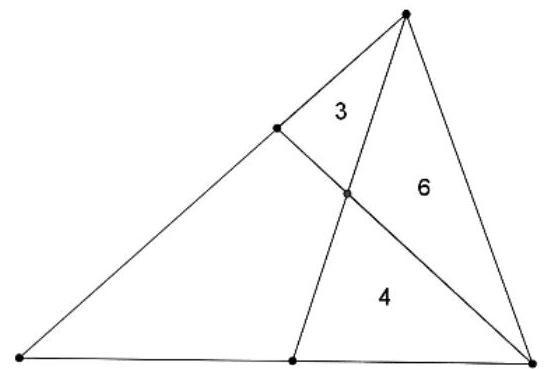
\includegraphics[max width=\textwidth, center]{2024_11_21_b4be4f78af681b2945efg-1}
  \item W trójkąt ostrokątny ABC wpisano kwadrat tak, że dwa jego wierzchołki należą do boku AB, a dwa pozostałe do pozostałych boków trójkąta. Udowodnij, że pole tego kwadratu nie przekracza połowy pola trójkąta ABC.
  \item Na szachownicy \(9 \times 9\) ustawiono 9 wież w ten sposób, że żadne dwie spośród nich nie zagrażają sobie. Każdą z tych figur przestawimy ruchem konika szachowego na inne pole. Czy da się to tak zrobić, żeby wieże dalej sobie nie zagrażały? Odpowiedź uzasadnij.
\end{enumerate}

\end{document}